\documentclass[a4paper,fullpack]{article}

% Font used is Latin-Modern (version of computer modern)
% http://www.gust.org.pl/projects/e-foundry/latin-modern
\usepackage{lmodern}
\usepackage{graphicx}
\usepackage{color}
\usepackage{hyperref}


\title{Internet of Coins\\[6mm]
\small{Hybrid Assets for Peer-to-Peer Inter-Blockchain Value Transfer}
}

\newcommand{\hyb}[1]{\ensuremath{\mathtt{ HYB }_{#1}}}
\newcommand{\TODO}{{\color{red}\texttt{TODO: }}}
\newcommand{\IDEA}{{\color{blue}\texttt{IDEA: }}}
\newcommand{\crypt}[1]{\ensuremath{ {\lbrace {#1} \rbrace} } }

\newcommand{\hybridd}{\texttt{hybridd}\, }
\newcommand{\stormwind}{\texttt{STORMWIND}\, }
\newcommand{\haystack}{\emph{Haystack}}

\makeindex

\begin{document}
\maketitle




\begin{abstract}
 A meta-protocol and blockchain integration solution for transacting value across different digital currency systems would allow for multiple decentralized financial platforms to exchange value and thus form a coherent cryptosphere, without needing intermediary financial institutions. Third party services currently assist users to exchange one form of digital cash or asset for another, but a trusted third party is still required to mediate these transactions. We propose a solution to the problem of isolated digital currency systems using a meta-level transfer protocol with an extendable design, making accessible any kind of blockchain-based economy or other digital cash system for cross-blockchain and inter-system transactions. A dynamic proof-of-allocation mechanism provides verification of solvency to any of the transferable assets on such a high-level platform, and makes it possible for anonymous allocation providers to earn rewards to be part of an autonomous, decentralized exchange system. Simultaneously, any network participant may act as an agent for the realization of an encrypted exchange of value between two peers. Information is transacted across the blockchains or digicash systems of the respective value-holders being traded, while node connections are directly negotiated without retaining or storing any records. As with Bitcoin, the network itself requires minimal structure, and messages are broadcast on a best effort basis. Swarm cryptography and multiple peer connections employ failover restructuring of transactions and messaging, and nodes can leave and rejoin the network at will, updating their allocation tables from any random node.
\end{abstract}


\section{Introduction}

Since the inception of Bitcoin, we have seen the rise of many digital cash descendants that either imitate or replicate the peer-to-peer version of electronic cash that Bitcoin was designed to be. Besides blockchain technology, decentralized asset exchanges\cite{counterparty} have been built to facilitate the issuing of virtual assets. Ledgerless \cite{opentransactions} systems have also been development, even before Bitcoin. While the existing solutions may function as intended, exchanges in value between these systems and blockchains is most often mediated through trusted third parties. This re-introduces the inherent weaknesses of the traditional trust based financial models into the realm of peer-to-peer digital currencies. In many cases this is no direct threat to the usage and trade of these currencies. Yet at the same time the different implementations of digital cash remain isolated from eachother, other than their exchange value relative to the Bitcoin. This exposes these currencies to price manipulation strategies that have the potential to drain value from these markets. \cite{panture}

What is needed is a hybrid asset and transfer system utilizing a modular and standardized peer-to-peer platform, to replace the trust model. A loosely coupled system\cite{EDA} allowing any two willing parties to transact assets cross-blockchain with each other, without the need for a trusted third party. Transaction methods that have no systemic boundaries and can operate cross-blockchain and inter-systemic, and may thus tie different value systems together. Through hybrid assets, loosely coupled financial systems create a cryptosphere that is immune to MITM (man-in-the-middle) intermediary control by trusted parties and stabilizes crypto-economies by enabling the value of smaller markets to be transferred into hybrid assets in the event of network destabilization. In this paper, we propose a solution to the digital economy diaspora using a peer-to-peer, distributed, inter-systemic and inter-blockchain exchange server to mediate the transfer of value between digital currency systems.


\section{Inter-Blockchain Transactions}

We define a hybrid asset as a blockchain-agnostic set of tokens\cite{coloredcoins} allocated on multiple digital value exchanges or multiple blockchains. The asset may gain a form of inherent value if its issuer decides to prove the asset's contextual value by either proof-of-burn\cite{proofofburn} or proof-of-stake\cite{proofofburn}. Asset holders on the hybrid network have either issued the asset themselves, or have obtained it on a decentralized asset exchange. Our proposed network daemon (hybridd) 'glues' crypto-assets and coins together by passing around datasets or tables - utilizing a FIFO (first-in-first-out) blockstream for sharing and verifying data - that contain identification information about each invidual blockchain-based asset, and rulesets that govern their relationship to form a hybrid asset. This allows for the creation of assets that have the flexibility to pass their value from blockchain to blockchain, or system to system. An owner may transfer an asset to another blockchain by cryptographically proposing a transaction to which any other peer on the hybridd network may respond. To make these kinds of transactions possible, an allocator node on the network must have allocated a certain amount of assets or coins to be used for inter-blockchain transactions. Information about allocators that hold such amounts is shared through the network, and constitutes a dynamic POA (proof-of-allocation) table for each network node.

Communication between exchanging peers goes through an anonymous swarm of nodes that act as an escrow for the network. The nodes in this group use \haystack cryptography to ensure impartial activity as a swarm or hive. Explained in simple terms haystack works as follows. Both the allocator of a transaction (Alice) and the initiator (Bob) receive public addresses from a swarm escrow (we will call this group Cipher). Cipher makes available a multitude of public keys created by each individual member of the swarm. These keys form multisignature transaction keys\cite{multisig} when combined. For a more detailed description of this mechanism, see section 10.

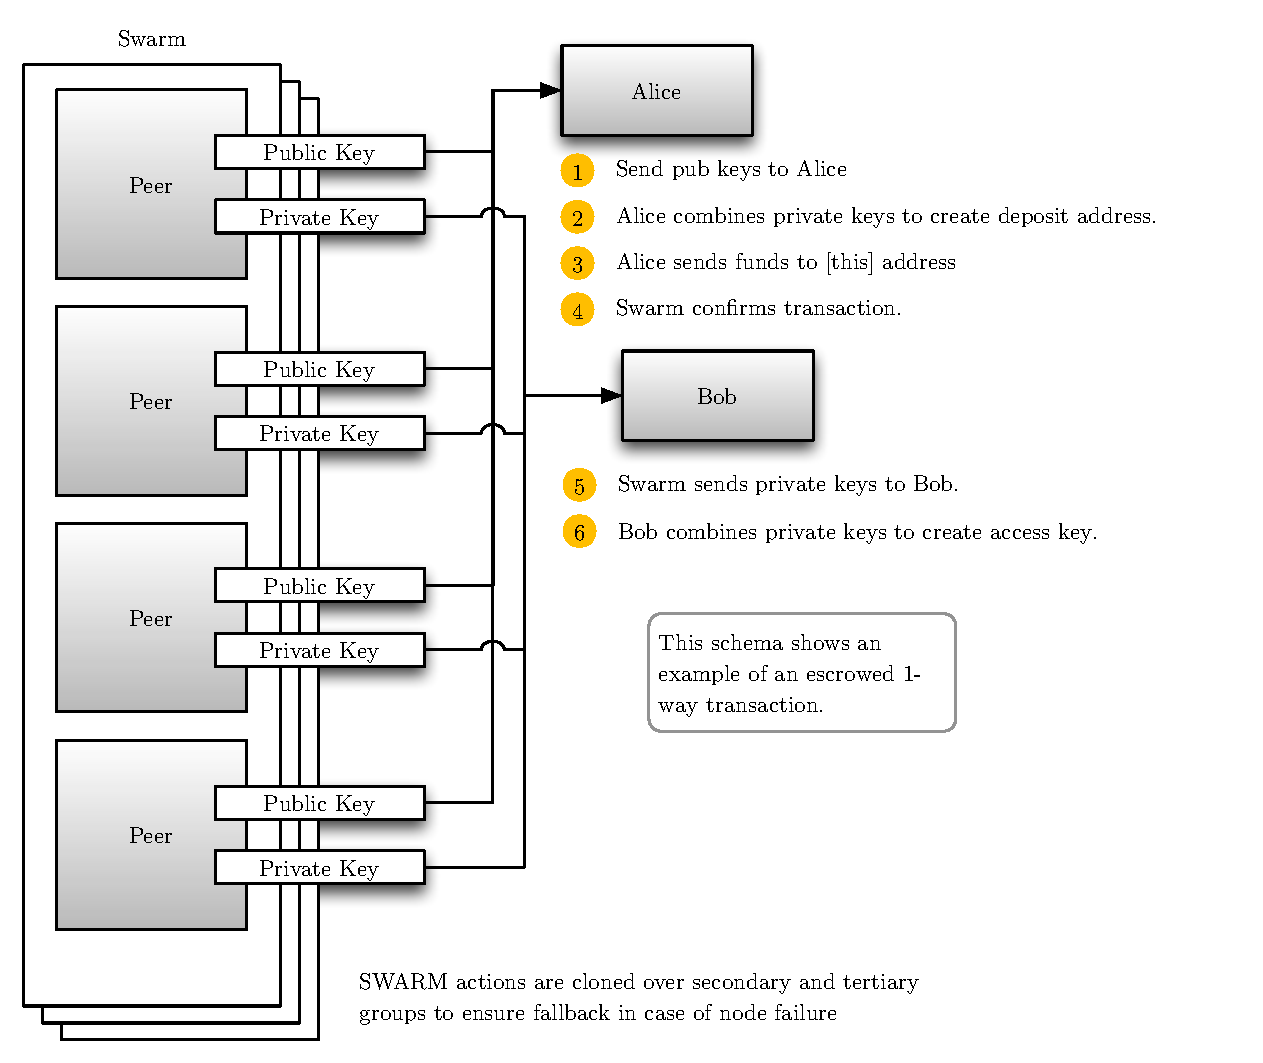
\includegraphics[width=.9\textwidth]{images/1-way-transaction.pdf}


\section{Meta Server}

To be able to integrate technically incompatible value models and peer-to-peer blockchains, we must take the approach of creating a peer-to-peer meta server that loosely couples current digital value systems on a high level, and makes trusted third parties unnecessary. This meta-structure should provide hooks to which abstract concepts of digital value systems and blockchain technologies can be connected and integrated. Modular and open extensions facilitate the implementation of different kinds of hybrid value systems in pluggable modules to unify the overlapping functionalities of different blockchains and ledgerless systems.

The meta-server networking daemon (hybridd) must use a concise and practical encrypted communications protocol and functions modularly  on top of existing anonymous routing networks such as, for example, TOR\cite{tor}, I2P\cite{i2p}, or GNUnet\cite{gnunet}, using their networks as a transport. This makes it more difficult to trivially identify individual node IP addresses, and makes NAT and firewall traversal easier. Peer ID's and their public keys are shared among peers as data in a distributed hash table\cite{dht}. Each PeerID is subject to a lease, and the entries of the peertable are intermittently verified by the participants in the network and timestamped.

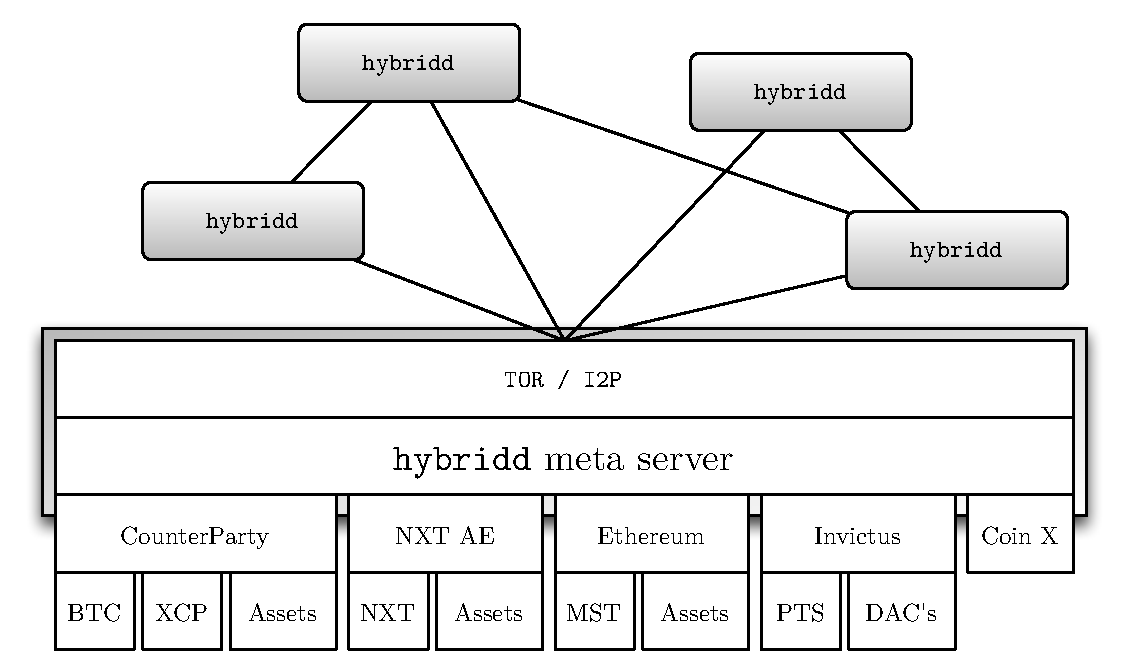
\includegraphics[width=.9\textwidth]{images/forumimg_hybridd.pdf}


\section{Proof-of-Allocation}

To make sure peers are able to determine the viability of a transaction before initiating one, we will need to use a proof-of-allocation (POA) table. To ensure the information in this table is correct, peers perform ledger auditing and verification when they have compatible active modules to access the blockchain or system on which the allocated amount is recorded. The POA table can be interpreted by individual nodes to ensure which transaction combinations are possible and viable, and which peers are eligible for transaction.

In the example you will notice there are four addresses holding the asset \stormwind, according to the POA table. Each node with access to NXT-AE (NXT) and CounterParty (XCP) blockchains is able to verify the allocated amount of assets specified in the table. By combining the information from a local database, a node can deduct that in this example the asset \stormwind has an allocation of 96,425 on the NXT blockchain and 49,500 on the XCP blockchain. The total proof-of-allocation amount would in this case be simply 145,925 units.

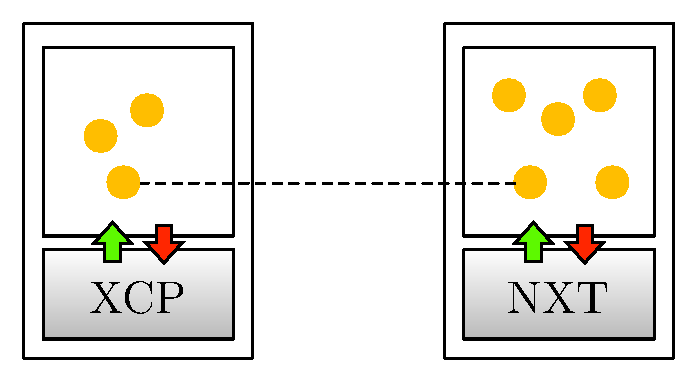
\includegraphics[width=.9\textwidth]{images/forumimg_valuetokens.pdf}

\section{Network}

The meta-server can theoretically bootstrap the network over any existing darknet. As previously mentioned, we will use TOR as our example. The bootstrapping process would be as follows:

\begin{enumerate}
\item New nodes consult their latest PeerID table to connect to 8 other peers
\item Each node contacts the oldest peers of its PeerID table to determine their status
\item Each node verifies the POA table where possible using its extensions
	    for connecting to other blockchains
\item When a node mediates as an escrow, it verifies the transacting peers,
	    mediates the transaction and updates the POA table
\item Each node updates its peers with its latest PeerID and POA tables
\item Nodes accept other PeerID and POA tables, verify and merge them with their own
\item Tables are sorted and pruned and only diffs of the data are shared with other peers
\end{enumerate}

Essentially the meta server provides an access and control communications layer on top of existing blockchains, or light-clients. This means \hybridd can be run on full blockchains or connect to API's for value transfer. Whatever the user prefers and has resources for. In the case of enough storage space, access to blockchains would be preferred. The following figure shows an example layout of how \hybridd could be bootstrapped into the networks.

As the figure implies, the possibilities for inter-blockchain transactions opens a plethora of decentralized trading options and asset combinations. Competitive crypto-platforms become cooperative economic ecosystems in which users and communities have freedom to innovate indiscriminately. Large changes to individual blockchains or RPC API's can be adapted to by the hybridd network simply by rewriting one of its extensions, whether concerning high-level transacting or low-level atomic cryptography. Smaller, declining cryptocurrencies can be bound together in hybrid assets giving survivability and exchange flexibility to these coins.


\section{Incentive}

In a transaction we have an initiator and a responder. Responders, more aptly called allocators, are network participants and asset holders who have allocated their assets for trading. When initator Alice starts a transaction, the amount of assets she receives from allocator Bob will always be a little less than the amount she sends. In this way the allocator has an incentive to support the liquidity of the market and survivability of the network. The ratio for conversion is yet to be defined, but for now defaults to: $1N : 0.999N$.  The allocator retains a small amount, and thus is rewarded for providing Alice with an instant migration of her assets between systems. The costs of conversion are default very low: between $0.1\%$ and $0.2\%$, or the lowest possible denomination of value in a specific asset. Costs of conversion, however, can also be set to another amount by the network, to define an autonomously organized context for optimal liquidity. This should make large transactions relatively inexpensive, while microtransactions are also decentrally regulated to avoid abuse on the network.

The more allocators appear on the network, the more competition they have amongst eachother to be chosen for a transaction, lowering the incentive for popular coins, while at the same time attracting allocators to abandoned blockchains. This balances out the amount of allocators between systems, yet still brings in enough responders to keep the network active as a whole and its assets liquid.

Perhaps, for instance, an allocator may be able to provide services for some blockchains, but not for others. If there are a great amount of allocators for the Bitcoin blockchain, but only a few for NXT, the Bitcoin allocators will relatively be less rewarded and the NXT allocators more rewarded for their services over time. This balances out the incentive towards individual services, and their supply and demand for individual blockchains.


\section{Unified Asset Descriptor}

Information about hybrid assets is passed around the network in signed arrays called unified-asset-descriptors (UAD). They contain the combined asset ID's, minimum and maximum cost of conversion, bcrypt sums thereof, further descriptive information, and are signed by the creator of the hybrid asset. This makes it possible for individual nodes to verify that an asset cannot be hijacked by anyone other than the issuer. Based on the existence of a signed unified asset descriptor, the lease of a PeerID in the shared table is periodically renewed.

Certain aspects of a UAD can be changed, while other things cannot. Linked assets may not be removed from a UAD once added for over 48 hours to protect the stakeholders of a hybrid asset. Adding new assets to become part of the hybrid, however, is not prohibited. This makes it possible for a hybrid asset to evolve and become part of more blockchains at a point in time beyond its inception. The description of a hybrid asset may also be changed to reflect intelligible updates to the asset's constitution.

Changes to an asset are temporarily recorded and buffered in a FIFO blockstream with reserved active data space and at least several historic revisions. This gives possibilities to revert the asset changes to previous states if necessary. Again, decoupling an internal asset from the UAD is only possible within 48 hours of committing the change. A small blockstream keeps the meta-server light enough for anyone with several gigabytes of diskspace to make use of it. Downloading multiple blockchains on one computer may be more than enough of a challenge for an average user. Let's not make the pain any worse.


\section{Cross-Blockchain Distributed Autonomous Organizations}

Many crypto-asset and cryptocurrency teams claim to have a working platform for distributed autonomous organizations (DAO), however, the most flexible and powerful platforms for this seem currently (2014.12.09) to be Ethereum, Counterparty and NXT. Many other platforms rely on rudimentary scripting to give a minimal service level of distributed autonomy.

In itself \hybridd contains no platform for DAO operations. Instead we want to facilitate the efforts that are already available to us on other blockchain platforms. Considering another option would be to create an Ethereum extension to tap into the distributed power of its DAO platform. An Ethereum contract could then autonomously make decisions and relay the results back into the hybrid assets blockstream to create cross-blockchain services.

Extending into DAO territory can also be done on other platforms. This, however, depends largely on the motivations of module developers. In any case, reinventing the wheel would be a waste of time and resources, while combining the power of both hybrid assets and any truly DAO enabled platform leverages the possibilities of both, and can make DAO's truly cross-blockchain without relying on a trusted party.


\section{Value and Allocation Theory}

When issuing a hybrid asset we must take into account the necessary allocation overhead to ensure the assets are liquid and transferrable to other systems and blockchains. This overhead may have the effect of inflating the price of the asset, however, as more allocators enter the market the opposite may also be true. Let's do a little contemplation on value and allocation to anticipate the effects of allocation reliance and resulting behaviour of market participants in more extreme market conditions.

If part of a hybrid asset becomes scarce in the market, it could theoretically become subject to deflation on any of its host blockchains. For example: if we issue the hybrid asset APPLES on NXT-AE, Ethereum and Counterparty\cite{counterparty}, and are looking to ensure at least $30\%$ allocation, we need enough incentive for participants in the network to allocate such an amount. The incentive is nominally provided by the maximum percentual cost of conversion by the asset issuer, and – in most cases – provides enough allocators for cross-blockchain liquidity, because of the incentive mechanism.

As long as prices on separate blockchains remain tied to common market ranges, allocations should autonomously balance out because of the effect of demand and supply in the markets. However, if for some reason many holders of a hybrid asset choose to exit one of the individual host platforms and flee into another, this may create an imbalance in price for the asset between chains. Also the mass-abandonment of a host platform by users could effectively cause the perceived value of the asset on that specific platform to become unstable. In such extreme circumstances allocation resources could be exhausted.

Usually allocation service providers in the \hybridd network will have enough incentive to keep on staking more allocated funds in order to return the market to balance. Perhaps some may seek to repair the allocation shortage by trading over other exchanges; thereby taking some risk to reap profits. Additionally, a shortage of allocators will make for increased profits among the few that are left. These will attempt to process all transactions that now have no place to be handled elsewhere.

Our thought experiment makes evident the hybrid assets ecosystem invites participants to become allocators that balance our supply and demand, thereby creating a self-regulated decentralized market.


\section{Haystack Transactions}

\subsection{Overview}

Multisignature transactions use private and public keys. These keys are correlated cryptographic numbers which can be added or multiplied. In a multisignature transaction a public key corresponding to a private key, is simultaneously the sum of multiple public keys that are directly correlated to multiple private keys that also form the correlating private key when added up.

In a haystack transaction the public keys generated by the swarm are sent around to all members of the swarm, and also to Alice and Bob. Every transaction participant collects these multisignature keys and combines them to form escrow addresses to which Alice and Bob are to send their funds. As soon as the transactions are done the funds of Alice and Bob will be stored on public keys to which no party has access. Each individual in the swarm has only part of the entire private key combination, and Alice and Bob neither have a way of knowing the private key they need to redeem these funds. Their value is effectively locked on the network, until the swarm decides to release the corresponding private keys by way of a decentralized consensus mechanism. This only happens after the swarm has verified and confirmed the transactions of Alice and Bob on the blockchain, and releases corresponding private multisignature keys to Alice and Bob to enable them to redeem the value they are entitled to.

We are currently doing further research into the security of this method of exchange. Currently the approach proves to be pragmatic, due to the fact that the private keys needed by Alice and Bob can be released to them only after the confirmation of their transactions. Yet at the same time they cannot be used by the escrow swarm (Cipher) to influence the transaction itself. In case of a defector or saboteur node within the swarm there exists a deduplication method to make sure any individual peer cannot hold a private key hostage and thus effectively burn the escrowed funds. In that case another member of the swarm can release enough information to recreate a missing private key. This information cannot be used, however, to recreate the entire multisignature key by one individual member of the swarm alone.

The anonymous third party has no influence on the value of the exchange being done between the two exchanging parties, except for verifying, and releasing the transactions of both peers. In case of failure (a node member of Cipher drops offline) or a timeout, both Alice and Bob receive any necessary keys from failover peers, as the swarm employs deduplication to ensure the haystack transaction can be completed.

\subsection{Notation}

\subsubsection{Setting}

We are dealing with two block-chains, $X$ and $Y$, both of which:

\begin{itemize}
\item support multi-signature transactions
\item carry the hybrid asset
\end{itemize}

To be specific on which block-chain a hybrid asset lives we write \hyb{X}.

Our usual suspects are

\begin{description}
	\item[Alice] Offers to swap \hyb{Y} for \hyb{X}, she is called the \emph{allocator}.
	
	\item[Bob] has \hyb{Y} and wants \hyb{X}. He \emph{initiates} a transaction with Alice to swap his \hyb{Y} for her \hyb{X}.
	
	\item[Cipher] A trust-less third party that operates as an escrow service.
\end{description}

Given a value $x$ we write $\crypt{x}_K$ to denote $x$ encrypted with key $K$.

We use $(K_a, PK_a)$ to denote a keypair $a$ consisting of
$PK_a$, the public key of a pair $a$ and $K_a$, the private key.

\subsubsection{Protocol}

Bob has \hyb{Y} and wants \hyb{X}.

Bob finds an allocator on the network willing to swap his \hyb{Y} for \hyb{X}.
Alice responds and they form a contract stating what is exchanged by whom:

\[
s = \langle B, A, Y, X \rangle
\]

\subsubsection{Decentralized escrow}

This contract is sent to $C$ and we want $C$ to respond with:

\begin{description}
\item[first] Two addresses $\alpha$ and $\beta$ where \hyb{X} and \hyb{Y} should be send too
\item[then] Once $\alpha$ and $\beta$ contain the funds, a pair of keys is released by $C$ that transfers ownership of $\alpha$ to Bob and $\beta$ to Alice.
\item[alternatively] If either of $\alpha,\beta$ doesn't contain the required hybrid assets after some time, a pair of keys is released that gives Alice ownership of $\alpha$ again, same for bob, aborting the swap.
\end{description}

\subsubsection{Multisignature approach}

\subsubsection{Publish target address}

Suppose we have $N$ nodes and let each node $n$ generate two key-pairs,
one for each of the two addresses $\alpha, \beta$

\[
	(K_n^\alpha, PK_n^\alpha, K_n^\beta, PK_n^\beta)
\]

Each node keeps their $PK$ private and shares $K_n^\alpha$ and $K_n^\beta$.

When all $N$ keys are received we can construct the target addresses $\alpha, \beta$.
\[
	\alpha \equiv \prod K_n^\alpha
\]

These addresses need to be public, because they are to be monitored by each node.

\subsubsection{Release access keys}

When monitoring the two addresses, at the next tick there are two situations:

\begin{description}
\item[Succes] $\Rightarrow$ publish $\langle \crypt{K_n^\beta}_{PK_A}, \crypt{K_\alpha}_{PK_B} \rangle$
\item[Abort] $\Rightarrow$ publish $\langle \crypt{K_n^\alpha}_{PK_A}, \crypt{K_\beta}_{PK_B} \rangle$
\end{description}

Like before, when all $N$ keys are received we can construct the private keys and access the address $\alpha$ or $\beta$. First decode each $\crypt{K_n^\beta}_{PK_A}$ into $K_n^\beta$, then just combine

\[
	K_\alpha \equiv \prod K_n^\alpha
\]


\section{Guarantor Transactions}

Some platforms may never support multisignature transactions. Take for instance some of the dying cryptocurrencies that have recently considerably dropped in value and hashingpower. Swapping value between these systems would seem impossible without using a trusted third party. However, by using a guarantor transaction we can make impossible for allocator Alice to cheat on a transaction without being punished for it by the swarm. This type of transaction is also referred to as a moderated non-multisignature block-chain transaction.

To solve the dilemma of not having multisignature transactions at our disposal, we make use of a guarantor transaction method to give both transacting parties enough incentive to play out a transaction fairly. Before such a transaction can take place, the allocator is summoned by the swarm to place a deposit on a separate, multisignature capable block-chain. This deposit is more valuable than the amount being transacted, and the swarm holds it in escrow until the transaction on the other blockchains is finished. On success, the deposit is sent back to the allocator. In the event of foul play, the private key to this amount is sent to the wronged party. This would cause the allocator more loss than gain, and gives a strong incentive to play fair.

This transaction method should only be used as a fallback, since it can certainly be more easily exploited than a multisignature transaction. As blockchains always have some delay before payments are confirmed, Cipher can monitor to see if both parties have sent funds to eachother. The slowest blockchain determines when both transactions have been broadcast into the networks. The guarantor transaction method will make it undesirable for the allocator to sabotage transaction, and gives a form of insurance to the initiating client, but we deem it an inferior method compared to a multisignature haystack transaction.

Notation for this work is to be expanded upon.


\section{Conclusion}

We have proposed a decentralized network transaction system for hybrid assets and decentralized transactions without relying on trusted third parties. Initially we defined decentralized assets, and described the threat of isolated cryptocurrencies and blockchains, with only centralized actors for exchanging value between these systems. To solve this, we proposed a peer-to-peer network operating over darknets to enable users to transact value across blockchains and value systems. 

By using multisignature transactions as a cryptographically secure method, advanced cryptography technology can be used for secure cross-blockchain transactions. In case of value systems without multisignature support, we have the possibility to fall back to transactions using the haystack transaction method. The network is self-balancing, anonymized and robust, using threshold cryptography for swarm escrow functionality. Nodes share information about hybrid assets across the network. Nodes can leave and rejoin the network at will, sharing proof-of-allocation tables containing data about the allocations and capabilities of each individual node. Value allocation and transactions are automatically managed by the allocating nodes, hybrid assets have a one-on-one inter-blockchain value definition, and prices for transacting value, supply and demand are decentrally market driven.


\section{References}

\bibliography{internetofcoins}{}
\bibliographystyle{plain}

\end{document}
